\documentclass{beamer}
%\usecolortheme{beaver}

\usepackage{amssymb, amsmath}
%\usepackage[all]{xy}

\usepackage{alltt}
\usepackage{pslatex}
\usepackage{epigraph}
\usepackage{verbatim}

\usepackage{graphicx}
\usepackage{latexsym}
\usepackage{array}
\usepackage{comment}
\usepackage{makeidx}
\usepackage{listings}
\usepackage{indentfirst}
\usepackage{verbatim}
\usepackage{color}
\usepackage{soul}
\usepackage{url}
\usepackage{xspace}
%\usepackage{fontspec}
%\usepackage{xunicode}
%\usepackage{xltxtra}
%\usepackage{xecyr}
\usepackage{hyperref}
%\usepackage[english]{babel}
%\usepackage[utf8]{inputenc}
%\setmainfont[Mapping=tex-text]{DejaVu Serif}
%\setsansfont[Mapping=tex-text]{DejaVu Sans}
%\setmonofont[Mapping=tex-text]{DejaVu Sans Mono}
%\usepackage{polyglossia}
%\setdefaultlanguage{russian}
\usepackage{stmaryrd}
\usepackage[normalem]{ulem}
\usepackage{xcolor}
\usepackage{wasysym}

\usepackage{amsmath, amsthm, amssymb}
\usepackage{graphicx}
\usepackage{euscript}
\usepackage{mathtools}
\usepackage{tikz}
\usepackage{tikz-qtree}
\usepackage{bchart}

\newcommand\redsout{\bgroup\markoverwith{\textcolor{red}{\rule[0.5ex]{2pt}{0.9pt}}}\ULon}

\makeatletter
\begin{comment}
\newcolumntype{e}[1]{%--- Enumerated cells ---
   >{\minipage[t]{\linewidth}%
     \NoHyper%                Hyperref adds a vertical space
     \let\\\tabularnewline
     \enumerate
        \addtolength{\rightskip}{0pt plus 50pt}% for raggedright
        \setlength{\itemsep}{-\parsep}}%
   p{#1}%
   <{\@finalstrut\@arstrutbox\endenumerate
     \endNoHyper
     \endminipage}}

\newcolumntype{i}[1]{%--- Itemized cells ---
   >{\minipage[t]{\linewidth}%
        \let\\\tabularnewline
        \itemize
           \addtolength{\rightskip}{0pt plus 50pt}%
           \setlength{\itemsep}{-\parsep}}%
   p{#1}%
   <{\@finalstrut\@arstrutbox\enditemize\endminipage}}

\AtBeginDocument{%
    \@ifpackageloaded{hyperref}{}%
        {\let\NoHyper\relax\let\endNoHyper\relax}}
\end{comment}

\makeatother

\definecolor{shadecolor}{gray}{1.00}
\definecolor{darkgray}{gray}{0.30}

\let\emptyset\varnothing
\newcommand{\set}[1]{\{#1\}}
\newcommand{\angled}[1]{\langle {#1} \rangle}
\newcommand{\fib}{\rightarrow_{\mathit{fib}}}
\newcommand{\fibm}{\Rightarrow_{\mathit{fib}}}
\newcommand{\oo}[1]{{#1}^o}
\newcommand{\inml}[1]{\mbox{\lstinline{#1}}}
\newcommand{\goal}{\mathfrak G}
\newcommand{\inmath}[1]{\mbox{$#1$}}
\newcommand{\sembr}[1]{\llbracket{#1}\rrbracket}
\newcommand{\inbr}[1]{\left<{#1}\right>}
\newcommand{\bigslant}[2]{{\raisebox{.2em}{$#1$}\left/\raisebox{-.2em}{$#2$}\right.}}

\newcommand{\withenv}[2]{{#1}\vdash{#2}}
\newcommand{\ruleno}[1]{\eqno[\textsc{#1}]}
\newcommand{\trule}[2]{\dfrac{#1}{#2}}

%\setlength{\epigraphwidth}{.55\textwidth}

\definecolor{light-gray}{gray}{0.90}
\definecolor{dark-green}{rgb}{0.30, 0.60, 0.1}
\definecolor{dark-red}{rgb}{0.80, 0.1, 0.1}

\newcommand{\graybox}[1]{\colorbox{light-gray}{#1}}

\newcommand{\nredrule}[3]{
  \begin{array}{cl}
    \textsf{[{#1}]}& 
    \begin{array}{c}
      #2 \\
      \hline
      \raisebox{-1pt}{\ensuremath{#3}}
    \end{array}
  \end{array}}

\newcommand{\naxiom}[2]{
  \begin{array}{cl}
    \textsf{[{#1}]} & \raisebox{-1pt}{\ensuremath{#2}}
  \end{array}}

\lstdefinelanguage{ocaml}{
keywords={let, begin, end, in, match, and,
function, try, with, class, object, method, of, rec, repeat, until,
while, not, do, done, as, val, inherit, module, sig, @type, struct, 
if, then, else, open, virtual, new, fresh},
sensitive=true,
basicstyle=\small,
commentstyle=\scriptsize\rmfamily,
keywordstyle=\ttfamily\bfseries,
identifierstyle=\ttfamily,
basewidth={0.5em,0.5em},
columns=fixed,
fontadjust=true,
literate={->}{{$\to$}}3 {===}{{$\equiv$}}1 {=/=}{{$\not\equiv$}}1 {|>}{{$\triangleright$}}3 {\&\&\&}{{$\wedge$}}2 {|||}{{$\vee$}}2 {^}{{$\uparrow$}}1,
morecomment=[s]{(*}{*)}
}

\lstset{
mathescape=true,
basicstyle=\small,
identifierstyle=\ttfamily,
keywordstyle=\bfseries,
commentstyle=\scriptsize\rmfamily,
basewidth={0.5em,0.5em},
fontadjust=true,
escapechar=!,
language=ocaml,
moredelim=[is][\ttfamily\color{blue}]{@}{@}
}

\begin{comment}
\lstdefinelanguage{ocaml}{
keywords={fresh, let, begin, end, in, match, type, and, fun, function, try, with, when, class,
object, method, of, rec, repeat, until, while, not, do, done, as, val, inherit,
new, module, sig, deriving, datatype, struct, if, then, else, open, private, virtual, include, @type},
sensitive=true,
commentstyle=\small\itshape\ttfamily,
keywordstyle=\ttfamily\underbar,
identifierstyle=\ttfamily,
basewidth={0.5em,0.5em},
columns=fixed,
fontadjust=true,
literate={->}{{$\to\;\;$}}3 {===}{{$\equiv$}}3 {=/=}{{$\not\equiv$}}3 {|>}{{$\triangleright$}}3,
morecomment=[s]{(*}{*)}
}

\lstset{
mathescape=true,
identifierstyle=\ttfamily,
keywordstyle=\bfseries,
commentstyle=\scriptsize\rmfamily,
basewidth={0.5em,0.5em},
fontadjust=true,
language=ocaml
}
\end{comment}
\sloppy

\newcommand{\miniKanren}{\texttt{miniKanren}\xspace}
\newcommand{\ocanren}{\texttt{OCanren}\xspace}
\newcommand{\ocaml}{\texttt{OCaml}\xspace}

\setbeamertemplate{footline}[frame number]
\setbeamertemplate{navigation symbols}{}
\setbeamertemplate{blocks}[rounded][shadow=true] 
\beamertemplateballitem

\setul{0.5ex}{0.3ex}
\setulcolor{blue}

\mode<presentation>{
  \usetheme{default}
}

\theoremstyle{definition}

\newtheorem{thm}{Theorem}[section] % the main one
% other statement types

% for specifying a name
\theoremstyle{plain} % just in case the style had changed
\newcommand{\thistheoremname}{}
\newtheorem{genericthm}[thm]{\thistheoremname}
\newenvironment{namedthm}[1]
  {\renewcommand{\thistheoremname}{#1}%
   \begin{genericthm}}
  {\end{genericthm}}

\title{Certified Semantics for miniKanren}

\author{
  \underline{Dmitry Rozplokhas}$^{1,3}$ \and Andrey Vyatkin$^2$ \and Dmitry Boulytchev$^{2,3}$
}

\institute[]{
\small{
  $^1$ Higher School of Economics, Russia \\
  $^2$ Saint Petersburg State University, Russia \\
  $^3$ JetBrains Research, Russia
}
}

\date{
   \vskip 1cm
   \small{
   \textbf{miniKanren and Relational Programming Workshop}\\
   August 22, 2019 \\
   Berlin, Germany}
}

\begin{document}
\begin{frame}[plain]
  \titlepage
\end{frame}



\begin{frame}{Motivation}

miniKanren is not a language, but a zoo:

\begin{itemize}
\item different logical constructions and extensions
\item different host languages and implementation details
\end{itemize}

\vskip8mm

Currently, we ought to believe different versions are consistent \\ w.r.t. each other

\vskip5mm

But have no means to prove it

\end{frame}



\begin{frame}{Motivation}

Also, there are some well-known observations about evaluation of miniKanren programs which are practically important

\vskip5mm

Most of them we can not prove formally:
\begin{itemize}
\item disjunction commutativity w.r.t. termination
\item conjunction commutativity w.r.t. answers
\end{itemize}

\vskip5mm

Some of them we can not formulate strictly:
\begin{itemize}
\item search completeness (``Any \underline{answer satisfying the relation} will be found in a finite time'')
\item notion of refutational completeness
\end{itemize}

\end{frame}



\begin{frame}{Motivation}

For that we would need formal semantics

\vskip10mm

\visible<2->{Today we will give you \textbf{two}!}

\end{frame}



\begin{frame}{Certified semantics}

Pen-and-paper specification are fragile (and quite boring to make)

\vskip5mm

Especially in our case, because:
\begin{itemize}
\item we work with (potentially) infinite objects
\item the proofs have a lot cases and a lot of details to track down
\end{itemize}

\vskip8mm

So we are doing it in Coq

\end{frame}



\begin{frame}{Talk outline}

\begin{enumerate}
  \item Basic language \visible<2->{\textcolor{blue}{+ specification in Coq}}
  \vskip6mm
  \item Denotational semantics \visible<2->{\textcolor{blue}{+ specification in Coq}}
  \vskip6mm
  \item Operational semantics \visible<2->{\textcolor{blue}{+ specification in Coq}}
  \vskip6mm
  \item Equivalence of the semantics \visible<2->{\textcolor{blue}{+ proof mechanization in Coq}}
\end{enumerate}

\end{frame}



\begin{frame}{Language in open space}

The simplest version to reason about

\vskip8mm

$ \begin{array}{ccll}
  term & ::= & \phantom{\mid} var & \quad \textit{\textcolor{darkgray}{(variable)}} \\
           &       & \mid constr (term_1, \dots, term_n) & \quad \textit{\textcolor{darkgray}{(constructor)}} \\ \\
  goal  & ::= & \phantom{\mid} term_1 \equiv term_2 & \quad \textit{\textcolor{darkgray}{(unification)}} \\
           &       & \mid goal_1 \land goal_2 & \quad \textit{\textcolor{darkgray}{(conjunction)}} \\
           &       & \mid goal_1 \lor goal_2 & \quad \textit{\textcolor{darkgray}{(disjunction)}} \\
           &       & \mid fresh \;\; (var) \;\; goal & \quad \textit{\textcolor{darkgray}{(existential variable introduction)}} \\
           &       & \mid rel (term_1, \dots, term_n) & \quad \textit{\textcolor{darkgray}{(relational call)}} \\
\end{array} $

\end{frame}


\begin{frame}{Language in Coq}

We add some restrictions which do not change language expressivity, but make everything much easier:
\vskip5mm
\begin{itemize}
\item Only binary and nullary constructors

\begin{center}
\lstinline|Triple(A, B, C)|

$\downarrow$

\lstinline|Constr(Triple, Cons(A, Cons(B, Cons(C, Nil))))|
\end{center}

\vskip3mm
\item Only unary relations

\begin{center}
\lstinline|eq$^o$ $\;$ x y = x === $\;$ y|

$\downarrow$

\lstinline|eq$^o$ $\;$ args = fresh (x y) (args === $\;$ Cons(x, Cons(y, Nil)) &&& x === $\;$ y)|
\end{center}

\end{itemize}

\end{frame}



\begin{frame}[fragile]{Language in Coq}

For bindings we use \textbf{Higher-order abstract syntax}

\begin{lstlisting}
Fresh (fun x -> Unify (Var x) (Cst 0))
\end{lstlisting}

\vskip5mm

\begin{itemize}
\item[+] No fuss with syntactic variables
\item[+] Suitable inductive principle out of the box
\item[-] No ``coherence'' of bindings, so we need to require it explicitly
\item[-] Some other well-known higher-order pitfalls
\end{itemize}

\end{frame}



\begin{frame}{Denotational semantics}

We use the standard approach for logic PLs --- \emph{the least Herbrand model}

\vskip10mm

Alternatively, we could just describe a conversion into a set of definite clauses and use its model

\vskip5mm

But:

\begin{itemize}
\item we would need to define the model for definite clauses in a certified way
\item the conversion may be non-trivial for language with extensions
\end{itemize}

\end{frame}



\begin{frame}{Denotational semantics: objective}

\begin{center}
$\llbracket$relation in program$\rrbracket$ $=$ relation over the set of ground terms
\end{center}

\pause

\vskip5mm

Representing functions:

\begin{center}
${\mathfrak f} \colon$ logical variables $\to$ ground terms
\end{center}

Semantics of a goal:

\begin{center}
$\sembr{goal} \subset \{ {\mathfrak f} \mid {\mathfrak f}$ is a representing function$\}$
\end{center}

\pause

\vskip5mm

Completeness condition: only free variables of a goal are restricted

\[\forall {\mathfrak f}, {\mathfrak f'}:  {\mathfrak f}\big{|}_{FV(g)} = {\mathfrak f'}\big{|}_{FV(g)}, \quad {\mathfrak f} \in \sembr{g} \Leftrightarrow {\mathfrak f'} \in \sembr{g}\]

%$ \forall\alpha\not\in FV\,(g) \quad \forall d \in \mathcal{D} \quad \forall\mathfrak{f} \in \sembr{g}, $

%$ \exists \mathfrak{f'} \in \sembr{g}: \;\; \phantom{\forall \beta \neq \alpha: \;\;} \mathfrak{f'}\,(\alpha)\; = d \qquad \wedge $

%$ \phantom{\exists \mathfrak{f'} \in \sembr{g}: \;\;} \forall \beta \neq \alpha: \;\; \mathfrak{f'}\,(\beta)\; = \mathfrak{f}\,(\beta)\; $

\end{frame}



\begin{frame}{Denotational semantics: goal constructors}

$\llbracket t_1 \equiv t_2 \rrbracket_{\Gamma} = \{{\mathfrak f} \mid \overline{\mathfrak f}(t_1) = \overline{\mathfrak f}(t_2) \}$

\vskip2mm

\qquad (where $\overline{\mathfrak f}$ applies ${\mathfrak f}$ to all logical variables in the term)

\vskip5mm

$\llbracket g_1 \land g_2 \rrbracket_{\Gamma} = \llbracket g_1 \rrbracket_{\Gamma} \cap \llbracket g_2 \rrbracket_{\Gamma}$

\vskip5mm

$\llbracket g_1 \lor g_2 \rrbracket_{\Gamma} = \llbracket g_1 \rrbracket_{\Gamma} \cup \llbracket g_2 \rrbracket_{\Gamma}$

\vskip5mm

$\llbracket fresh \; (x) \; g \rrbracket_{\Gamma} = \llbracket g[a/x] \rrbracket_{\Gamma} \uparrow a, \quad a \notin FV(g)$

\vskip2mm

\qquad (where $\uparrow a$ ``forgets'' all restrictions on logical variable $a$)

\end{frame}



\begin{frame}{Denotational semantics: example}

\[ \begin{array}{lc}
\visible<1->{\sembr{\mbox{\lstinline|fresh y . ($\alpha$ === y) $\,\wedge\,$ (y === Zero)|}}_{\Gamma}} & \visible<2->{=} \\[3mm]
\visible<2->{(\sembr{\mbox{\lstinline|($\alpha$ === $\beta$) $\,\wedge\,$ ($\beta$ === Zero)|}}_{\Gamma})\uparrow\beta} & \visible<3->{=} \\[3mm]
\visible<3->{(\sembr{\mbox{\lstinline|$\alpha$ === $\beta$|}}_{\Gamma} \,\cap\, \sembr{\mbox{\lstinline|$\beta$ === Zero)|}}_{\Gamma})\uparrow\beta} & \visible<4->{=} \\[3mm]
\visible<4->{(\{\mathfrak{f}\mid \overline{\mathfrak{f}}\,(\alpha)=\overline{\mathfrak{f}}\,(\beta)\} \,\cap\, \{\mathfrak{f}\mid \overline{\mathfrak{f}}\,(\beta)=\overline{\mathfrak{f}}\,(\mbox{\lstinline|Zero|})\})\uparrow\beta} & \visible<5->{=} \\[3mm]
\visible<5->{(\{\mathfrak{f}\mid \mathfrak{f}\,(\alpha)=\mathfrak{f}\,(\beta)\} \,\cap\, \{\mathfrak{f}\mid \mathfrak{f}\,(\beta)=\mbox{\lstinline|Zero|}\})\uparrow\beta} & \visible<6->{=} \\[3mm]
\visible<6->{(\{\mathfrak{f}\mid \mathfrak{f}\,(\alpha)=\mathfrak{f}\,(\beta)=\mbox{\lstinline|Zero|}\})\uparrow\beta} & \visible<7->{=} \\[3mm]
\visible<7->{\{\mathfrak{f}\mid \mathfrak{f}\,(\alpha)=\mbox{\lstinline|Zero|}\}} & \\[3mm]
\end{array} \]

\end{frame}



\begin{frame}{Denotational semantics: relational calls}

Building the least Herbrand model

\vskip5mm
\begin{center}

$ \Gamma \colon name \to $ args $ \to $ set of representing functions

\[ \llbracket r(t_1, \dots, t_n) \rrbracket_\Gamma = \Gamma(r)(t_1, \dots, t_n) \]

\vskip10mm

$ \mathcal{F}(\Gamma) = r \mapsto args \mapsto \llbracket$ body of the relation $r$ with $ args \; \rrbracket_\Gamma $

\[ \Gamma_0 = fix \; \mathcal{F} \]

\vskip-4mm

\[ \llbracket g \rrbracket  = \llbracket g \rrbracket_{\Gamma_0}  \]

\end{center}

\end{frame}



\begin{frame}[fragile]{Denotational semantics: notes on specification}

Representing functions defined simply as Coq functions:
\begin{lstlisting}
Definition repr_fun : Set := var -> ground_term.
\end{lstlisting}

\vskip5mm

Denotational semantics defined as inductive proposition:
\begin{lstlisting}
Inductive in_denotational_sem_goal :
    goal -> repr_fun -> Prop := ...
\end{lstlisting}

\vskip5mm

The least fixpoint semantic is implicitly provided by inductive definition

\vskip5mm

The proof of arbitrarity of choice of fresh variable is unexpectedly cumbersome

\end{frame}



\begin{frame}{Operational semantics}

Should reflect program execution for some \emph{realistic} implementation

\vskip3mm

In particular, should capture search termination

\vskip8mm

Described as a \emph{deterministic Labeled Transition System \\ with observable answers}

\end{frame}



\begin{frame}{Operational semantics: transition system}

States:

\[nSt \;=\; \langle goal, subst, counter \rangle \;\;|\;\; nSt \oplus nSt \;\;|\;\; nSt \otimes goal \] 
\[St \;=\; nSt \;\;|\;\; \Diamond\]

\vskip5mm

Transitions:

\begin{center}
$St \xrightarrow{} St \qquad $ or $ \qquad St \xrightarrow{(subst, counter)} St$
\end{center}

\pause

\vskip8mm

\begin{tabular}{ll}
Terminating execution: & $\inbr{g, \epsilon, n} \xrightarrow{} St_1 \xrightarrow{(\sigma_0, n_0)} St_2 \xrightarrow{(\sigma_1, n_1)} \Diamond$ \\
Diverging execution: & $\inbr{g, \epsilon, n} \xrightarrow{} St_1 \xrightarrow{(\sigma_0, n_0)} St_2 \xrightarrow{(\sigma_1, n_1)} St_3 \xrightarrow{} \dots$ \\
\end{tabular}

\end{frame}



\begin{frame}{Operational semantics: rules for goals}

\begin{itemize}

\item For unification we use Most General Unifier

$\inbr{t_1 \equiv t_2, \sigma, n} \xrightarrow{} \Diamond , \, \, \nexists\; mgu\,(t_1, t_2, \sigma)$

$\inbr{t_1 \equiv t_2, \sigma, n} \xrightarrow{(mgu\,(t_1, t_2, \sigma),\, n)} \Diamond$

\pause

\vskip4mm

\item For conjunction and disjunction we construct states of corresponding types

$\inbr{g_1 \lor g_2, \sigma, n} \xrightarrow{} \inbr{g_1, \sigma, n} \oplus \inbr{g_2, \sigma, n}$

$\inbr{g_1 \land g_2, \sigma, n} \xrightarrow{} \inbr{ g_1, \sigma, n} \otimes g_2$

\pause

\vskip4mm

\item For fresh we update the counter

$\inbr{fresh \; (x) \; g, \sigma, n} \xrightarrow{} \inbr{g\,[\bigslant{\alpha_{n + 1}}{x}], \sigma, n + 1}$

\pause

\vskip4mm

\item For relational invokation we take the body of the relation

$\dfrac{r\;=\;\lambda\,x_1\dots x_{k_i}\,.\,g}{\inbr{r\,(t_1,\dots,t_{k_i}),\sigma,n} \xrightarrow{} \inbr{g\,[\bigslant{t_1}{x_1}\dots\bigslant{t_{k_i}}{x_{k_i}}], \sigma, n}}$

\end{itemize}

\end{frame}



\begin{frame}{Operational semantics: rules for interleaving}
    
The search is parallel in sum

\begin{center}
\begin{tabular}{lll}

$\dfrac{s_1 \xrightarrow{r} \Diamond}{(s_1 \oplus s_2) \xrightarrow{r} s_2}$ &

$\dfrac{s_1 \xrightarrow{r} s'_1}{(s_1 \oplus s_2) \xrightarrow{r} (s_2 \oplus s'_1)}$ &

... \\

\end{tabular}
\end{center}

\vskip4mm

and sequential in product

\begin{center}
\begin{tabular}{lll}

$\dfrac{s \xrightarrow{(\sigma, n)} \Diamond}{(s \otimes g) \xrightarrow{} \inbr{g, \sigma, n}} $ &

$\dfrac{s \xrightarrow{(\sigma, n)} s'}{(s \otimes g) \xrightarrow{} \inbr{g, \sigma, n} \oplus (s' \otimes g)}$ &

... \\

\end{tabular}
\end{center}

\pause

\vskip5mm

Some basic properties we can prove here:

\begin{itemize}
\item In a disjunction an answer will be found iff it will be found in either of disjuncts
\item In a disjunction the search terminates iff the search terminates in both disjuncts
\end{itemize}

\end{frame}



\begin{frame}[fragile]{Operational semantics: note on certification}

It is well-known, that the textbooks algorithms for MGU computation are not structurally recursive w.r.t. argument terms \\ $\Rightarrow$ \\ Direct encoding in Coq is problematic

\vskip5mm

We define it as a proposition
\begin{lstlisting}
Inductive MGU : term -> term -> option subst -> Set := ...
\end{lstlisting}

\vskip5mm

but still need well-founded induction (on the number of free variables) to prove its definitional properties.

\end{frame}



\begin{frame}[fragile]{Operational semantics: notes on specification}

Transition relation is encoded as an inductively defined proposition:
\begin{lstlisting}
Inductive eval_step : n_state -> label -> state -> Set := ...
\end{lstlisting}

\pause

\vskip5mm

Traces are defined coinductively:
\begin{lstlisting}
CoInductive trace : Set := ...

CoInductive op_sem : state -> trace -> Prop := ...
\end{lstlisting}

\vskip3mm

but some of their properties make sense only when defined inductively
\begin{lstlisting}
Inductive in_trace : answer -> trace -> Prop := ...

Inductive finite : trace -> Prop := ...
\end{lstlisting}

\end{frame}



\begin{frame}{Semantics equivalence}

First, we need to relate two kinds of results

\begin{center}

$ [\sigma] = \{ \overline{\mathfrak f} \circ \sigma \mid {\mathfrak f}$ is a representing function$\}$

\vskip5mm

$\llbracket s \rrbracket_{op} = \bigcup\limits_{(\sigma, n) \in Tr_s} [\sigma]$
\end{center}

\pause

\begin{namedthm}{Interleaving search soundness and completeness}
If $FV(g) \subset \{\alpha_1,\dots,\alpha_n\}$,

$
\{ \mathfrak{f}|_{\{\alpha_1,\dots,\alpha_n\}} \mid \mathfrak{f} \in \sembr{\inbr{g, \epsilon, n}} \}
=
\{\mathfrak{f}|_{\{\alpha_1,\dots,\alpha_n\}} \mid \mathfrak{f} \in \sembr{\inbr{g, \epsilon, n}}_{op} \}
$
\end{namedthm}
\begin{proof}
Generalize the statement and use nested structural induction
\end{proof}

\end{frame}



\begin{frame}{Generalizations for the proof}

\begin{enumerate}

\item Denotational semantics of states

\begin{itemize}

\item does not need to have any intuitive interpretation

\item is introduced only for proof to go smoothly

\end{itemize}

\item Bounded denotational semantics $\sembr{\bullet}^i$

\vskip3mm

Unfolds definitions of relations only $i$ times

\vskip3mm

$\sembr{g}^0 = \emptyset$

\begin{lemma}
$\sembr{g} \subset \cup_i \sembr{g}^i$
\end{lemma}
\begin{proof}
By the definition of the least fixed point from Tarski-Knaster theorem
\end{proof}


\end{enumerate}

\end{frame}



\begin{frame}{Note on certification: the proof of semantics equivalence}

It is rather long and all green!

\begin{tabular}{cc}
Generalized correctness & \hskip15mm Generalized completeness \\
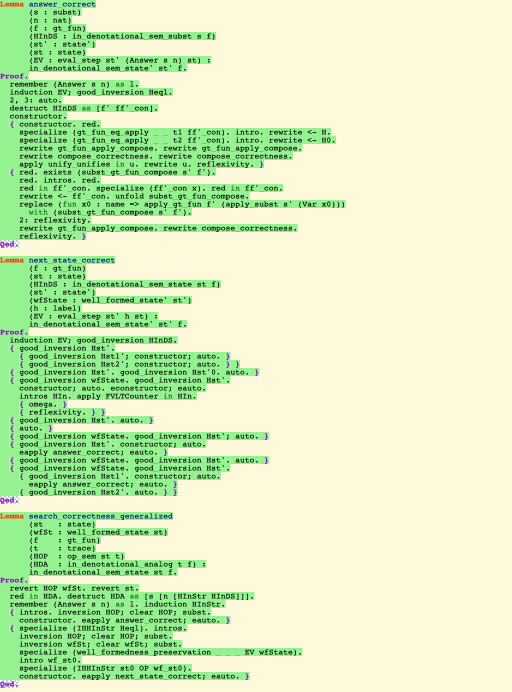
\includegraphics[scale=0.25]{correctness_proof.png} & \hskip15mm 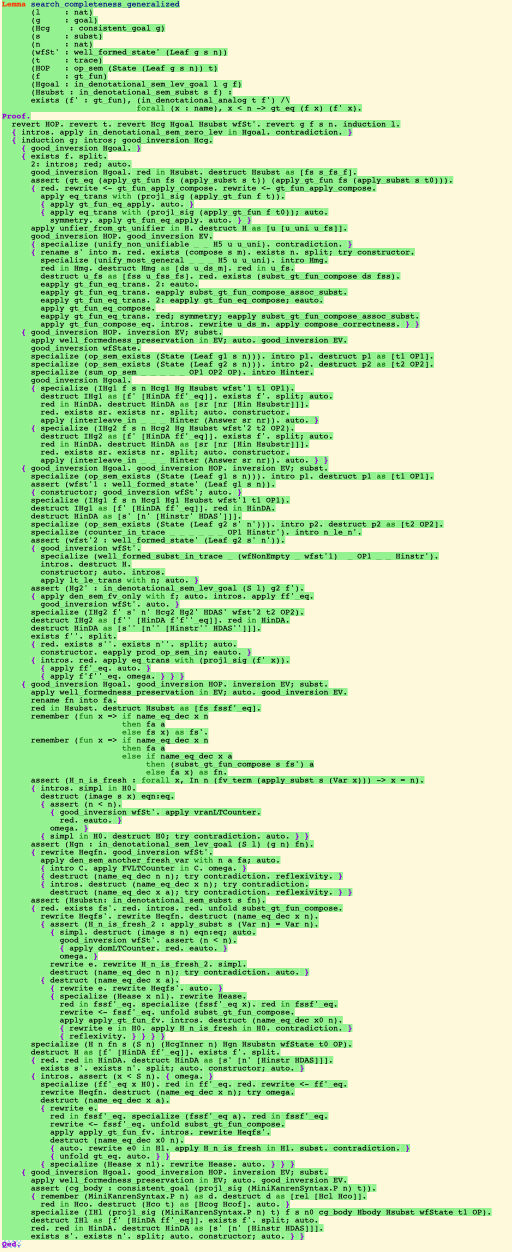
\includegraphics[scale=0.25]{completeness_proof.png} \\
\end{tabular}

\vskip5mm

Formalization revealed serious flaws in pen-and-paper proofs for both directions

\end{frame}



\begin{frame}{Corollary: correctness of program transformations}

Transformations which are invariant w.r.t. denotational semantics have the same result of evaluation (the set of answers):

\vspace{3mm}

\begin{itemize}
\item conjunction/disjunction commutativity,
\item distributivity,
\item fresh lifting,
\item \dots
\end{itemize}

\vspace{10mm}

Programs may be fearlessly converted into canonical form

\end{frame}



\begin{frame}{Conclusions}

\begin{itemize}

\item Two formal semantics for miniKanren

\vskip5mm

\item Equivalence result

\vskip5mm

\item Everything is certified in Coq

\vskip5mm

\item Correctness of certain transformations

\vskip5mm

\item (Uncertified) properties of certain relations

\end{itemize}

\end{frame}



\begin{frame}{Future work}

\begin{itemize}

\item Language extensions (primarily - disequality constraint)

\vskip6mm

\item A certified interpreter by extraction

\vskip6mm

\item Correctness of improved search strategies

\end{itemize}

\end{frame}

\end{document}
